\documentclass[12pt,a4paper]{article}
\usepackage[utf8]{inputenc}
\usepackage[russian]{babel}
\usepackage[OT1]{fontenc}
\usepackage{mathtools}
\usepackage{amsfonts}
\usepackage{amssymb}
\usepackage{enumitem}
\usepackage{alltt}
\usepackage{graphicx}
\usepackage{indentfirst}
\usepackage{caption}
\usepackage{float}
\usepackage{wrapfig}
\usepackage{physics}
\usepackage{multirow}
\usepackage{longtable}
\usepackage{amsmath,amsfonts,amssymb,amsthm,mathtools}
\usepackage{icomma}
\setlength{\parindent}{0.75cm}
\graphicspath{{pictures/}}
\DeclareGraphicsExtensions{.png, .jpg}
\usepackage[left=15mm,right=15mm,top=2cm,bottom=2cm]{geometry}
\author{Глотов Алексей}
\begin{document}
\newpage
\begin{center}
\footnotesize{{ГОСУДАРСТВЕННОЕ АВТОНОМНОЕ ОБРАЗОВАТЕЛЬНОЕ УЧРЕЖДЕНИЕ}\break
{ВЫСШЕГО ОБРАЗОВАНИЯ}
\break
{\bf {МОСКОВСКИЙ ФИЗИКО-ТЕХНИЧЕСКИЙ ИНСТИТУТ}}
\break
\small{(НАЦИОНАЛЬНЫЙ ИССЛЕДОВАТЕЛЬСКИЙ УНИВЕРСИТЕТ)}}
\break
\hfill \break
\hfill \break
\begin{center}
\normalsize{Кафедра общей физики}
\end{center}
\hfill \break
\hfill \break
\hfill \break
\hfill \break

\begin{center}
\normalsize {Лабораторная работа 5.1.1}
\end{center}
\hfill \break\\
\large{\textbf{Экспериментальная проверка уравнения Эйнштейна для фотоэффекта и определение постоянной Планка}}
\end{center}
\begin{flushleft}
\hfill \break
\hfill \break
\hfill \break
\hfill \break
\hfill \break
\hfill \break
\hfill \break
\hfill \break
\hfill \break
\hfill \break
\hangindent=10cm
\normalsize{Преподаватель:} \;\;\;\;
\normalsize{к.ф.-м.н. Юрьев Ю.В.}\\
\hfill \break
\normalsize{Обучающийся:} \;\;\;\;\;
\normalsize{Глотов А.А} \\
\hfill \break
\end{flushleft}
\hfill \break
\hfill \break
\hfill \break
\hfill \break
\hfill \break
\hfill \break
\hfill \break
\hfill \break
\hfill \break
\hfill \break
\hfill \break

\begin{center}
Долгопрудный \break
 2023
\end{center}

\thispagestyle{empty}


\newpage
\section{Введение}

\subsection{Аннотация}

Испусканием электронов фотокатодом, облучаемым светом называется фототоком. Фотоэффект может быть объяснён с помощью фотонной теории света. Фотон с энергией $\hbar \omega$ выбивает из металла электрон и сообщает ему определённую кинетическую энергию. 

Данная работа посвящена исследованию данного явления, направленное на определение постоянной Планка

\textbf{Цель работы:} экспериментально проверить уравнение Эйнштейна для фотоэффекта и определить значение постоянной Планка

\subsection{Теоретические сведения}

При столкновении фотона с электроном фотокатода энергия фотона полностью передается электрону, и фотон прекращает свое существование. Энергетический баланс этого взаимодействия для вылетающих электронов описывается уравнением
	
	\begin{equation}\label{energy balance}
	\hbar \omega = E_{max} + W
	\end{equation}
	
	\begin{wrapfigure}{l}{0.3\linewidth}
		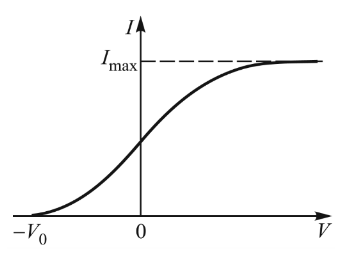
\includegraphics[width=\linewidth]{5.1.1-1}
		\caption{Зависимость фототока от напряжения на аноде фотоэлемента}
		\label{ris I(V)}
	\end{wrapfigure}
	
	Здесь $ E_{max} $ - максимальная кинетическая энергия электрона после выхода из фотокатода, $ W $ - работа выхода электрона из катода. Реально энергетический спектр вылетевших из фотокатода электронов непрерывен - он простирается от нуля до $ E_{max} $. 
	
	Для измерения энергии вылетевших фотоэлектронов вблизи фотокатода обычно располагается второй электрод (анод), на который подается задерживающий ($ V < 0 $) или ускоряющий ($ V > 0 $) потенциал. Качественный график зависимости фототока от напряжения представлен  (рис. \ref{ris I(V)})
	
	Максимальная кинетическая энергия $ E_{max} $ электронов связана с запирающим потенциалом $ V_0 $ очевидным соотношением $ E_{max} = eV_0 $. Тогда \eqref{energy balance} примет вид, называемый уравнением Эйнштейна:
	
	\begin{equation}\label{Einsteain}
	eV_0 = \hbar\omega - W 
	\end{equation}
	
	
	\begin{wrapfigure}{r}{0.3\linewidth}
	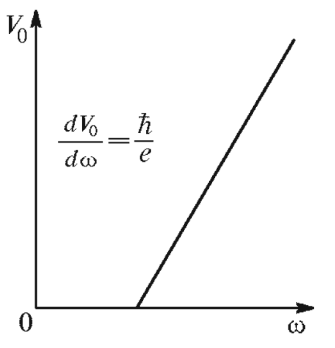
\includegraphics[width=\linewidth]{5.1.1-2}
	\vspace{-2ex}
		\caption{Зависимость запирающего потенциала
			от частоты света}
		\label{ris V(w)}
	\end{wrapfigure}
		
	
	Простейшая оценка зависимости тока от напряжения на наклонном участке приводит к следующему выражению
	
	\begin{equation}\label{sqrt I = V}
	\sqrt{I} \propto V_0 - V
	\end{equation}
	
Из \eqref{Einsteain} получим зависимость 
	
	\begin{equation}\label{V(w)}
	V_0 (\omega) = \dfrac{\hbar\omega - W}{e}
	\end{equation}

	Или, выписав ее в дифференциальной форме:
	
	\begin{equation}\label{dV/dw}
	\dfrac{dV_0}{d\omega} = \dfrac{\hbar}{e}
	\end{equation}


\section{Результаты измерений и обработка данных}

1. По спектральным линиям неона построим калибровочную зависимость угла монохроматора от длины волны

\begin{center}
\begin{tabular}{|c|c|c|c|c|c|c|c|c|c|c|c|c|c|}
\hline 
$\phi, ^\circ$ & 2536 & 2506 & 2442 & 2430 & 2400 & 2380 & 2370 & 2332 & 2326 & 2308 & 2296 & 2280  \\ 
\hline 
$\lambda$, нм & 703,2 & 692,9 & 671,7 & 667,8 & 659,9 & 653,3 & 650,7 & 640,2 & 638,3 & 633,4 & 630,5 & 626,7 \\ 
\hline 
$\phi, ^\circ$ & 2260 & 2238 & 2230 & 2208 & 2198 & 2178 & 2150 & 2138 & 2106 & 2092 & 1830 & 1792 & 1780 \\ 
\hline
$\lambda$, нм & 621,7 & 616,4 & 614,3 & 609,6 & 607,4 & 603,0 & 597,6 & 594,5 & 588,2 & 585,2 & 540,1 & 534,1 & 533,1  \\
\hline
\end{tabular} 
\end{center}

Здесь $\Delta \phi = 2 ^\circ$, длины волн берем без погрешности, считая табличные данные значительно точнее погрешности шкалы монохроматора

Калибровочный график по этим данным:

\begin{figure}[H]
	\begin{center}
		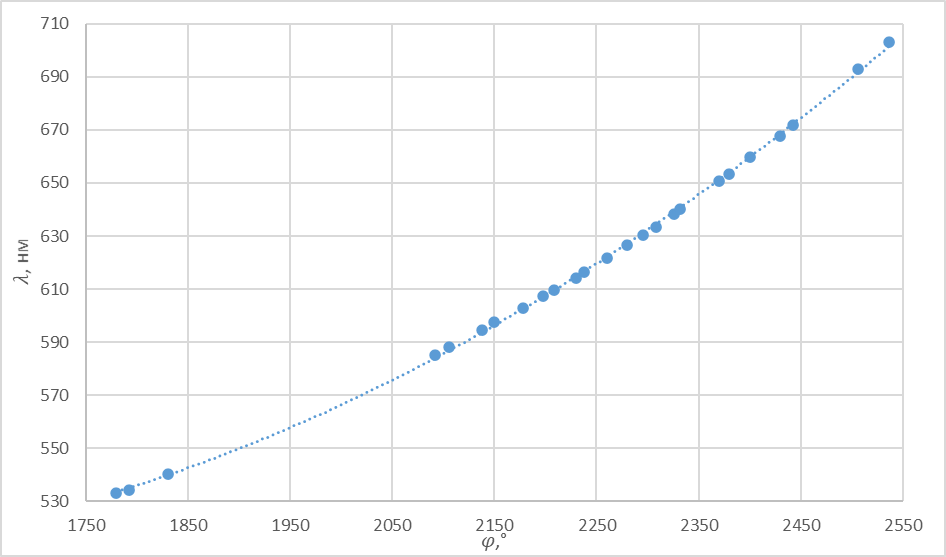
\includegraphics[width=14cm]{5.1.1-3}
		\caption{Калибровочный график}
	\end{center}
\end{figure}

Проведем 5 серий измерений для различных длин волн. Для упрощения перевода будем использовать длины волн спектра неона.

\begin{center}
\begin{tabular}{|c|c|c|c|c|c|c|c|c|c|}
\hline 
\multicolumn{2}{|c|}{703,2 нм} & \multicolumn{2}{|c|}{585,2 нм} & \multicolumn{2}{|c|}{533,1 нм} & \multicolumn{2}{|c|}{650,7 нм} &  \multicolumn{2}{|c|}{616,4 нм} \\ 
\hline 
V, В & I, у.е. & V, В & I, у.е. & V, В & I, у.е. & V, В & I, у.е. & V, В & I, у.е. \\ 
\hline 
-0,264 & -0,20 & -0,547 & 0,19 & -0,787 & 0,14 & -0,443 & 0,17 & -0,566 & 0,18 \\ 
\hline 
-0,155 & 0,33 & -0,408 & 0,28 & -0,666 & 0,18 & -0,352 & 0,24 & -0,451 & 0,24 \\ 
\hline 
-0,125 & 0,36 & -0,308 & 0,35 & -0,485 & 0,26 & -0,283 & 0,30 & -0,371 & 0,30 \\ 
\hline 
-0,048 & 0,46 & -0,226 & 0,42 & -0,320 & 0,36 & -0,234 & 0,35 & -0,308 & 0,35 \\ 
\hline 
-0,033 & 0,48 & -0,160 & 0,48 & -0,194 & 0,45 & -0,150 & 0,45 & -0,258 & 0,40 \\ 
\hline 
0,011 & 0,53 & -0,055 & 0,56 & -0,131 & 0,49 & -0,084 & 0,52 & -0,175 & 0,48 \\ 
\hline 
0,031 & 0,55 & 0,000 & 0,59 & -0,008 & 0,55 & -0,021 & 0,58 & -0,104 & 0,54 \\ 
\hline 
0,118 & 0,64 & 0,053 & 0,62 & 0,102 & 0,59 & 0,037 & 0,62 & -0,022 & 0,60 \\ 
\hline 
\end{tabular} 
\end{center}

По этим зависимостям построим графики: 

\begin{figure}[H]
\begin{minipage}[h]{0.48\linewidth}
\center{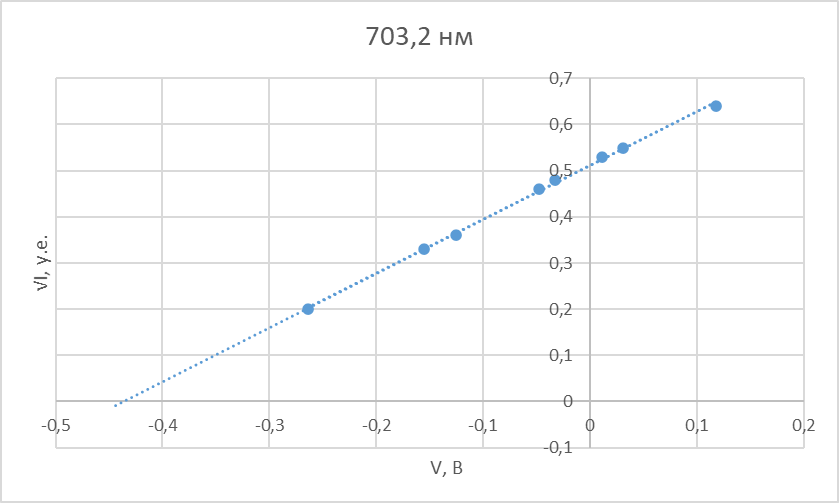
\includegraphics[width=1\linewidth]{5.1.1-4}} \\
\end{minipage}
\hfill
\begin{minipage}[h]{0.48\linewidth}
\center{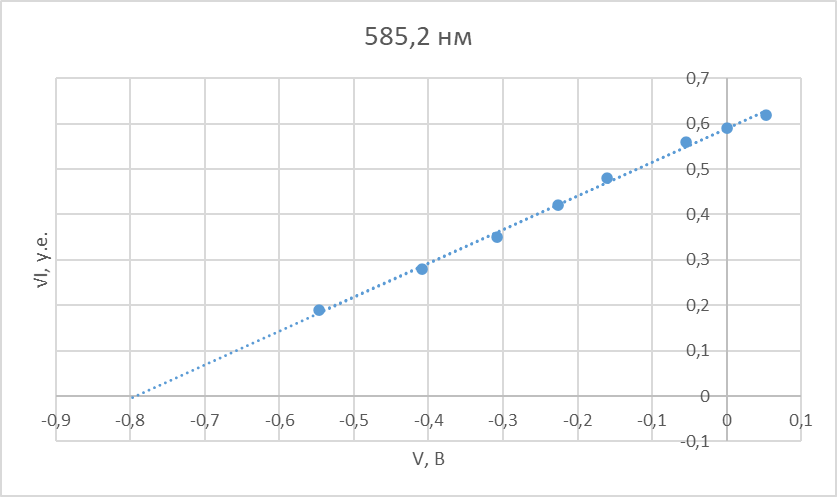
\includegraphics[width=1\linewidth]{5.1.1-5}} \\ 
\end{minipage}
\end{figure}

\begin{figure}[H]
\begin{minipage}[h]{0.48\linewidth}
\center{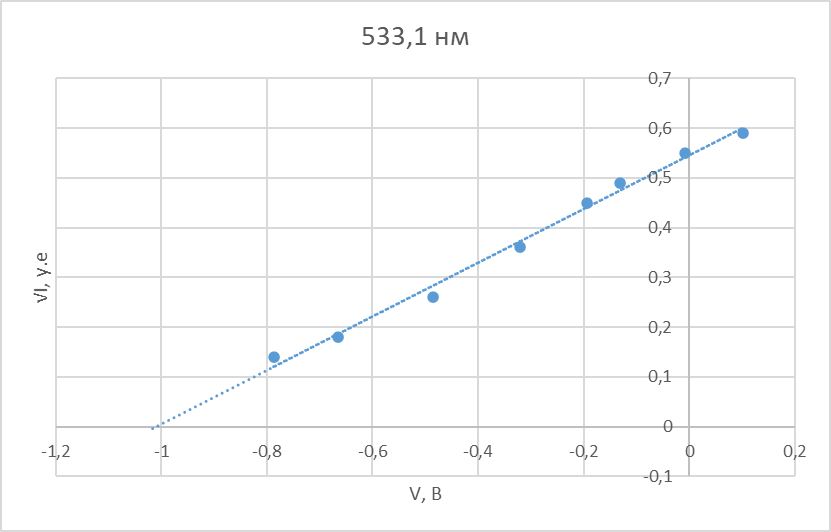
\includegraphics[width=1\linewidth]{5.1.1-6}} \\
\end{minipage}
\hfill
\begin{minipage}[h]{0.48\linewidth}
\center{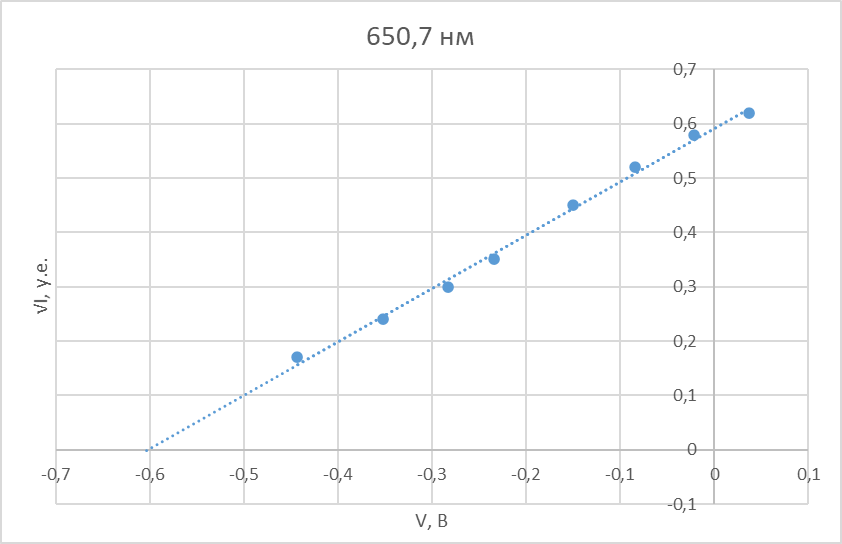
\includegraphics[width=1\linewidth]{5.1.1-7}} \\ 
\end{minipage}
\end{figure}

\begin{figure}[H]
\begin{minipage}[h]{0.48\linewidth}
\center{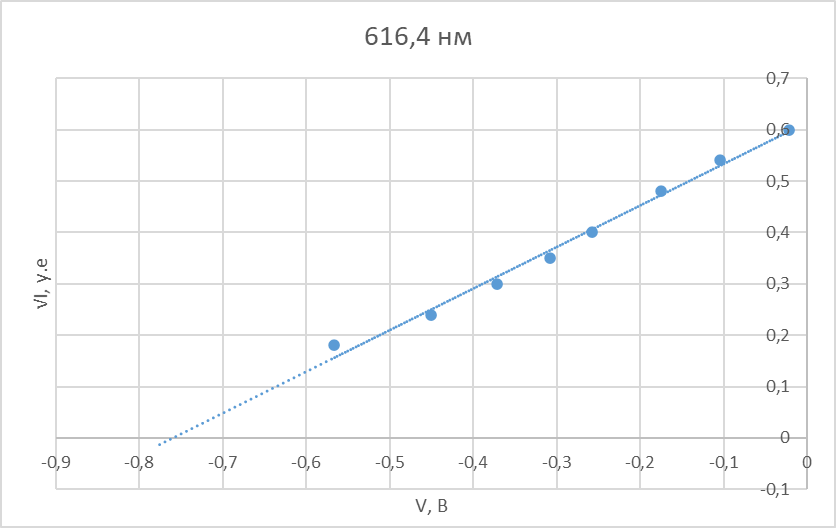
\includegraphics[width=1\linewidth]{5.1.1-8}} \\
\end{minipage}
\hfill
\begin{minipage}[h]{0.48\linewidth}
\center{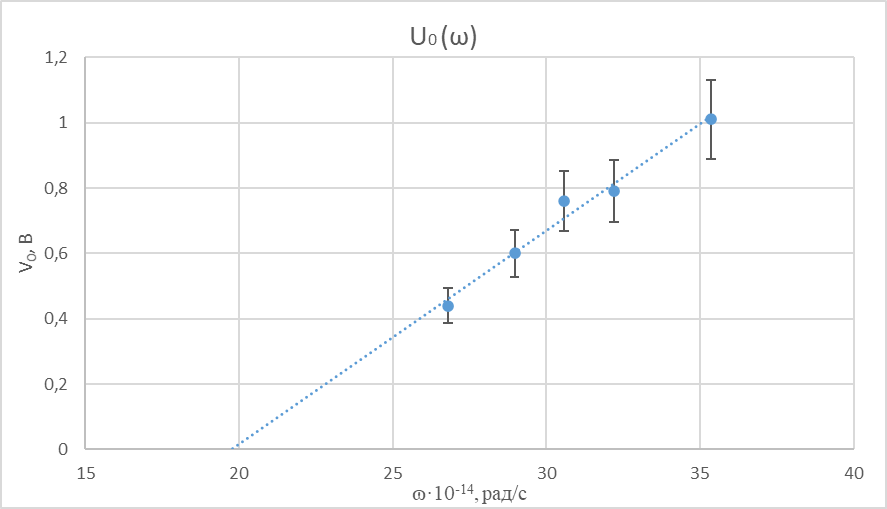
\includegraphics[width=1\linewidth]{5.1.1-9}} \\
\end{minipage}
\end{figure}

По МНК найдем запирающее напряжение для наших длин волн

\begin{center}
\begin{tabular}{|c|c|c|c|c|c|}
\hline 
$\lambda$, нм & 703,2 & 650,7 & 616,4 & 585,2 & 533,1 \\ 
\hline 
$\omega\cdot 10^{-14}$, рад/с  & 26.8 & 29.0 & 30.5 & 32.2 & 35.4 \\ 
\hline 
$U_0$, В & 0,44 $\pm$ 0.06 & 0.60 $\pm$ 0.08 & 0.76 $\pm$ 0.10 & 0.79 $\pm$ 0.11 & 1.01 $\pm$ 0.14 \\ 
\hline 
\end{tabular} 
\end{center}

Отсюда имеем:
\begin{center}
$h=2\pi e k = (6,53 \pm 0,98)\text{Дж}\cdot\text{с}$
\end{center}

	Красная граница фотоэффекта соответствует частоте, при которой $U_0$ = 0 :
\begin{center}
$\omega_\text{кр}=(2,0 \pm 0,3)\cdot 10^{15} $ рад/с
\end{center}

Отсюда:
\begin{center}
$\lambda_\text{кр} = 2\pi с / \omega_\text{кр} = 940 \pm 130$ нм
\end{center}

Работа выхода:
\begin{center}
$A_\text{вых} = \hbar \omega_\text{кр} = (1,3 \pm 0,2)$эВ
\end{center}



\section{Обсуждение результатов и выводы}
	В ходе работы мы экспериментально проверили уравнение Эйнштейна для фотоэффекта, а также определили значение постоянной Планка:
	
	\begin{center}
$h=2\pi e k = (6,53 \pm 0,98)\text{Дж}\cdot\text{с}$
\end{center}

Полученное значение оказалось достаточно близким к табличному

Красная граница фотоэффекта:

\begin{center}
$\lambda_\text{кр} = 2\pi с / \omega_\text{кр} = 940 \pm 130$ нм
\end{center}

Работа выхода для используемого фотокатода:

\begin{center}
$A_\text{вых} = \hbar \omega_\text{кр} = (1,3 \pm 0,2)$эВ
\end{center}	
	

\end{document}